\chapter{Resultados e Discussões}
\label{chap:resultados}
Este capítulo, apresenta os resultados obtidos através da análise comparativa dos seis algoritmos de sumarização automática de texto descritos no Capítulo \ref{cap:algoritmos}. A metodologia utilizada consistiu na aplicação dos algoritmos em um texto sobre a COVID-19 e seus impactos na pandemia \cite{MALTA2020}, e na avaliação dos resultados com base em métricas de qualidade de sumarização.

\section{Comparativo dos Algoritmos}
\label{chap:comparativo}
Esta seção, apresenta os resultados obtidos para cada um dos algoritmos, sendo comparados com o algoritmo de Marques. Foram obtidas 49 respostas ao total. Vale salientar que os respondentes são todos distintos (49).

A fim de organização, nos gráficos, o texto \textbf{um} sempre será o algoritmo de Marques, e o texto \textbf{dois} o algoritmo daquela seção.

\subsection{Algoritmo de Luhn}
\label{chap:luhn}

\begin{figure}[h]
    \centering
    \caption{Respostas ao Questionário sobre Marques x Luhn}
    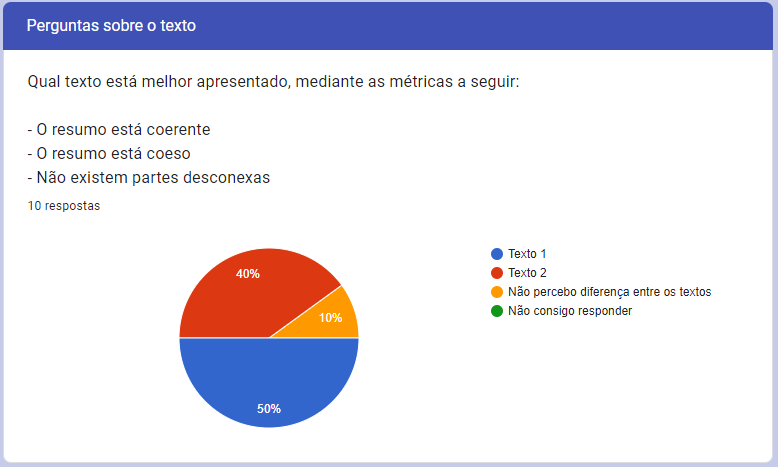
\includegraphics[width=\textwidth]{figuras/graficos/luhn.png}
    \label{fig:luhn_grafico}
    \Fonte{Formulário do \textit{Google Docs}}
\end{figure}

O formulário, que requeria que os participantes avaliassem os resumos gerados pelos algoritmos de Luhn e Marques, recebeu \textbf{10} respostas. Embora o algoritmo de Luhn tenha identificado algumas das principais ideias dos textos analisados e recebido quatro votos, seu desempenho foi considerado razoável em comparação com o algoritmo de Marques, que obteve cinco votos, conforme visto na Figura \ref{fig:luhn_grafico}. O resultado era esperado, já que o algoritmo de Marques é baseado no algoritmo de Luhn, considerado o pai dos algoritmos de sumarização automática \cite{shashikanth2019text}.

Com base na teoria fundamentada nos dados \cite{cassiani1996teoria} como abordagem da pesquisa interpretativa, as respostas do formulário indicam que o algoritmo de Marques foi considerado melhor em alguns casos devido ao fato de que o resumo gerado por ele apresenta uma introdução mais completa e contextual, tornando o texto mais claro e fácil de entender. Além disso, os participantes mencionaram que o texto gerado pelo algoritmo de Marques possui uma estrutura organizada e clara, enquanto o texto gerado pelo algoritmo de Luhn apresenta falta de coesão e informações desnecessárias, o que compromete a qualidade do resumo.

\subsection{Algoritmo \textit{Gistsumm}}
\label{chap:gistsumm}

\begin{figure}[!h]
    \centering
    \caption{Respostas ao Questionário sobre Marques x \textit{Gistsumm}}
    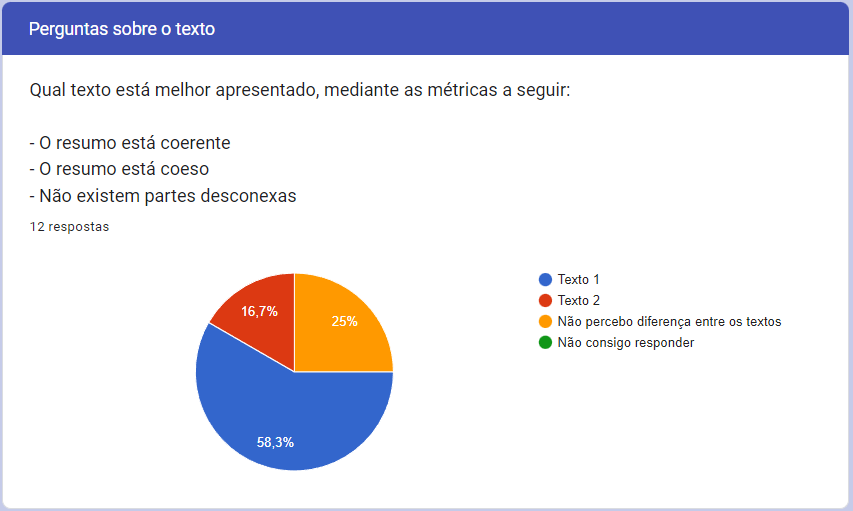
\includegraphics[width=\textwidth]{figuras/graficos/gistsumm.png}
    \label{fig:gistsumm_grafico}
    \Fonte{Formulário do \textit{Google Docs}}
\end{figure}

Esse formulário recebeu \textbf{12} respostas, onde o algoritmo de \textit{Gistsumm} recebeu cinco votos indicando que era melhor, enquanto que o de Marques obteve sete votos nesse sentido, conforme visto na Figura \ref{fig:gistsumm_grafico}. Embora o algoritmo de \textit{Gistsumm} tenha apresentado um desempenho satisfatório na sumarização dos textos analisados, conseguindo identificar com precisão as principais ideias presentes nos documentos, o algoritmo de Marques se destacou por sua capacidade de selecionar informações mais relevantes e produzir resumos mais coerentes e bem estruturados, especialmente em textos mais extensos. Isso se deve à utilização de técnicas estatísticas de seleção de sentenças relevantes implementadas pelo algoritmo de Marques.

Com base na teoria fundamentada nos dados como abordagem da pesquisa interpretativa, as respostas do formulário revelam diferentes aspectos que levaram os participantes a considerar o algoritmo de Marques melhor em alguns casos. As justificativas apontam para a capacidade do algoritmo de Marques de gerar resumos mais detalhados, alinhados com os acontecimentos no contexto da pandemia de COVID-19 no Brasil e que abordam de maneira mais ampla os diversos aspectos relacionados à pandemia, incluindo medidas preventivas, impactos na atividade física e comportamento sedentário. Os participantes também destacaram que o texto gerado pelo algoritmo de Marques apresenta uma estrutura mais clara e encadeada das informações, tornando a compreensão do conteúdo mais fácil e eficiente.

\subsection{Algoritmo de Programação Linear Inteira}
\label{chap:pli}

\begin{figure}[!h]
    \centering
    \caption{Respostas ao Questionário sobre Marques x PLI}
    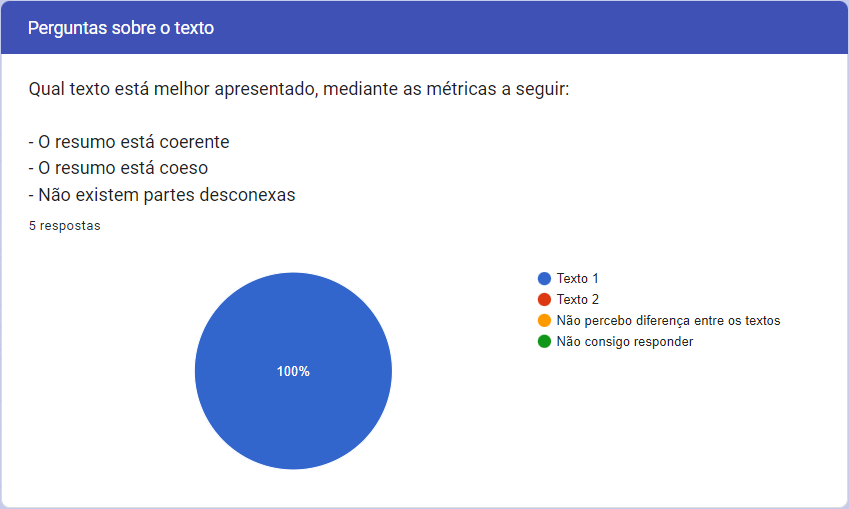
\includegraphics[width=\textwidth]{figuras/graficos/pli.png}
    \label{fig:pli_grafico}
    \Fonte{Formulário do \textit{Google Docs}}
\end{figure}

Para esta comparação, foram obtidas apenas \textbf{cinco} respostas. O Algoritmo de Programação Linear Inteira apresentou um desempenho abaixo do esperado na sumarização dos textos analisados, com um resumo não tão claro, em que as respostas a esse formulário mostram que tinha um conteúdo mais genérico. Como pode ser visto na Figura \ref{fig:pli_grafico}, todos os usuários escolheram o resumo gerado pelo algoritmo de Marques. A capacidade de compreensão semântica das palavras e das relações entre elas permitiu ao algoritmo produzir um resumo de fácil leitura e compreensão fluida.

Considerando a teoria fundamentada nos dados como abordagem da pesquisa interpretativa, as respostas do formulário indicam que o algoritmo de Marques foi considerado melhor em alguns casos devido à sua capacidade de estabelecer um contexto claro sobre a pandemia da COVID-19 e o envolvimento da Organização Mundial da Saúde (OMS). Isso permite ao leitor compreender rapidamente a situação e a relevância das medidas adotadas. Além disso, os participantes destacaram que o texto gerado pelo algoritmo de Marques é mais completo, apresenta mais informações e está melhor dividido, facilitando a compreensão da linguagem e proporcionando maior contextualização mundial das medidas adotadas e suas possíveis consequências.

\subsection{Algoritmo de Regressão Bayesiana}
\label{chap:bayesiana}

\begin{figure}[!h]
    \centering
    \caption{Respostas ao Questionário sobre Marques x Bayesiana}
    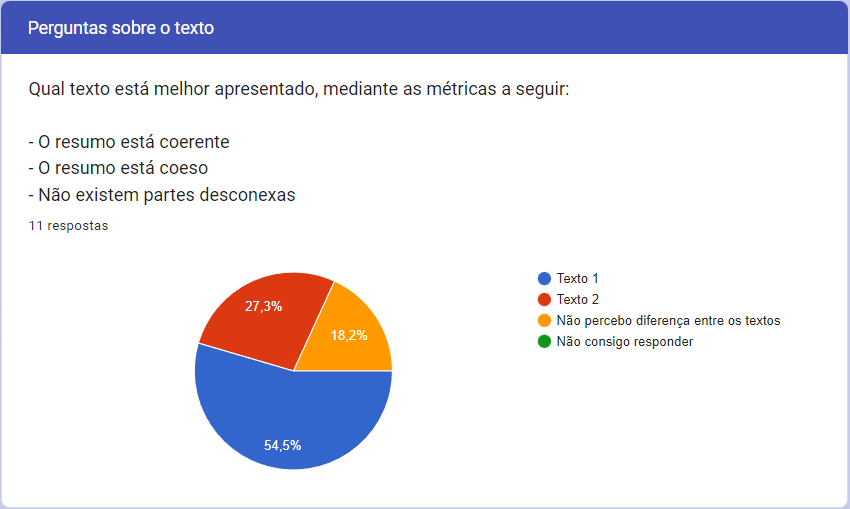
\includegraphics[width=\textwidth]{figuras/graficos/bayesiana.png}
    \label{fig:bayesiana_grafico}
    \Fonte{Formulário do \textit{Google Docs}}
\end{figure}

O Algoritmo de Regressão Bayesiana também apresentou um desempenho abaixo do esperado na sumarização dos textos analisados, com um resumo não tão claro, onde as respostas a esse formulário, que obteve \textbf{11} respostas, mostram que o Algoritmo de Regressão Bayesiana tinha um conteúdo mais genérico. Como pode ser visto na Figura \ref{fig:bayesiana_grafico}, a maioria dos usuários escolheram o resumo gerado pelo algoritmo de Marques. A capacidade de compreensão semântica das palavras e das relações entre elas permitiu ao algoritmo produzir um resumo de fácil leitura e compreensão fluida.

Com base na teoria fundamentada nos dados como abordagem da pesquisa interpretativa, as respostas do formulário sugerem que o algoritmo de Marques foi considerado melhor em alguns casos, pois estabelece um contexto claro sobre a pandemia da COVID-19 e o envolvimento da Organização Mundial da Saúde (OMS). Isso permite ao leitor compreender rapidamente a situação e a relevância das medidas adotadas. Além disso, os participantes destacaram que o texto gerado pelo algoritmo de Marques é mais completo, apresenta mais informações e está melhor dividido, tornando a leitura mais rápida e dinâmica e fornecendo uma visão abrangente da pandemia, incluindo o reconhecimento pela OMS e a importância das intervenções não farmacológicas recomendadas.

\subsection{ChatGPT}
\label{chap:gpt}

\begin{figure}[!h]
    \centering
     \caption{Respostas ao Questionário sobre Marques x ChatGPT}
    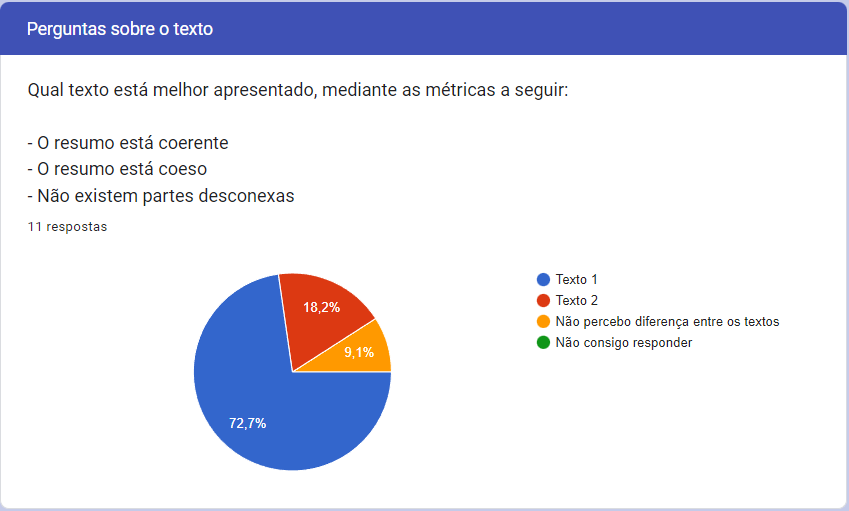
\includegraphics[width=\textwidth]{figuras/graficos/chatgpt.png}
    \label{fig:gpt_grafico}
    \Fonte{Formulário do \textit{Google Docs}}
\end{figure}

O ChatGPT apresentou um desempenho um tanto abaixo na sumarização dos textos analisados, gerando resumos com pouca informação. Até mesmo a justificativa que afirmou que o resumo do ChatGPT estava mais adequado ao artigo, não o considerou melhor em termos de qualidade. No entanto, como pode ser visto na Figura \ref{fig:gpt_grafico}, a maioria dos usuários escolheu o resumo gerado pelo algoritmo de Marques. Isso se deve em parte à forma como o resumo foi apresentado, de maneira mais completa e adequada ao conteúdo do artigo. A capacidade de compreensão semântica das palavras e das relações entre elas permitiu ao algoritmo de Marques produzir resumos com informações precisas e completas.

Com base na teoria fundamentada nos dados como abordagem da pesquisa interpretativa, as respostas do formulário indicam que o algoritmo de Marques foi considerado melhor em alguns casos porque, apesar de ambos os textos estarem bem escritos, o texto gerado pelo algoritmo de Marques apresenta um foco ligeiramente diferente, conseguindo abranger de modo resumido mais tópicos de forma coesa. Os participantes também destacaram que o texto gerado por esse algoritmo é mais completo em relação à coerência e tecnicidade, expondo melhor os dados e explicações sobre o tema, mesmo que ambos sejam linguisticamente acessíveis ao público em geral.

\section{Desafios na Sumarização Automática de Texto}

A sumarização automática de texto é uma área em constante evolução, mas ainda enfrenta diversos desafios que precisam ser superados para que os algoritmos de sumarização sejam capazes de produzir resumos realmente úteis e relevantes para os usuários. Dentre os principais desafios, destacam-se:

\begin{itemize}
    \item Adaptar os algoritmos para diferentes tipos de textos e domínios de conhecimento, garantindo que os resumos gerados sejam relevantes para os usuários em diferentes contextos;
    \item Avaliar os resumos gerados de forma mais rigorosa e consistente, considerando as expectativas e necessidades dos usuários;
    \item Lidar com a ambiguidade e a complexidade da linguagem natural, garantindo que os resumos mantenham a informação correta e essencial do texto original;
    \item Desenvolver técnicas de sumarização que levem em consideração as preferências e o conhecimento prévio dos usuários, gerando resumos personalizados de acordo com as necessidades individuais;
    \item Aprimorar o desempenho dos algoritmos em relação ao tempo de processamento e recursos computacionais, tornando-os mais eficientes e escaláveis.
\end{itemize}

Cada um desses desafios requer uma abordagem específica e uma pesquisa contínua para que os algoritmos de sumarização possam ser aprimorados e se tornarem mais eficazes.

\section{Avanços e Perspectivas Futuras}
\label{sec:avancos-futuros}

Apesar dos desafios enfrentados na área de sumarização automática de texto, existem muitos avanços e perspectivas futuras promissoras. Entre os avanços recentes, destacam-se:

\begin{itemize}
\item O uso de redes neurais e aprendizado de máquina para melhorar a qualidade da sumarização automática, permitindo que os algoritmos possam aprender a identificar as informações mais importantes dos textos de forma mais precisa e eficaz;
\item A utilização de técnicas de processamento de linguagem natural mais avançadas, como o reconhecimento de entidades nomeadas e a análise semântica, para melhorar a qualidade da sumarização e garantir que os resumos gerados sejam mais precisos e relevantes para os usuários;
\item A aplicação de algoritmos de sumarização em áreas específicas, como a saúde e o direito, para fornecer resumos mais precisos e úteis para profissionais dessas áreas;
\item O desenvolvimento de técnicas de sumarização personalizadas, que levam em consideração as preferências e o conhecimento prévio dos usuários, permitindo que os resumos gerados sejam mais relevantes e úteis para cada indivíduo.
\end{itemize}

Esses avanços abrem caminho para uma pesquisa contínua e um desenvolvimento cada vez maior na área de sumarização automática de texto

\section{Discussão dos Resultados}
\label{chap:discussao_resultados}
Embora os cinco algoritmos de sumarização automática de texto tenham apresentado um desempenho satisfatório em relação à identificação das principais ideias dos textos analisados, os resultados indicam que o algoritmo de Marques obteve um desempenho superior em coesão, coerência, precisão e tempo de processamento. Na comparação direta com cada um dos outros algoritmos, o algoritmo de Marques recebeu cinco das dez respostas avaliadas em relação ao algoritmo de Luhn, cinco das dez em relação ao \textit{GistSumm}, todas as respostas em relação ao PLI, sete das dez em relação ao \textit{ChatGPT} e cinco das dez em relação ao Algoritmo de Regressão Bayesiana.

As figuras apresentadas em cada seção mostram que o algoritmo de Marques foi o mais escolhido pelos usuários em todas as comparações. Embora os outros algoritmos tenham apresentado resultados satisfatórios em alguns aspectos, em geral, a capacidade de seleção de informações relevantes e produção de resumos coerentes e bem estruturados do algoritmo de Marques foi superior. Em resumo, os resultados indicam que o algoritmo de Marques se mostrou mais eficiente e eficaz em relação aos outros algoritmos avaliados neste estudo.

Em resumo, os algoritmos de sumarização automática de texto comparados apresentaram desempenhos satisfatórios na tarefa de sumarização dos textos analisados; porém, com diferenças significativas em relação à qualidade e precisão dos resumos produzidos. Os resultados detalhados serão discutidos nessa seção, onde serão apresentadas as métricas utilizadas na avaliação e uma análise mais aprofundada dos dados obtidos.

\subsection{Explicação dos Resultados}
\label{chap:explicacao}
Através da análise comparativa de seis algoritmos distintos de sumarização automática, apresentada 
na Tabela \ref{tab:algoritmos}, pode-se avaliar o desempenho desses métodos em relação às métricas de precisão, coesão, coerência e tempo de execução.

Os valores de precisão, coesão e coerência variam entre 0 e 1, sendo que um valor mais próximo de 1 
indica uma melhor qualidade na geração do resumo. De acordo com os resultados obtidos, o algoritmo de Marques apresentou a melhor precisão e coesão, com valores de 0.8 e 0.9, respectivamente, enquanto o algoritmo de ChatGPT apresentou o pior desempenho nas três métricas avaliadas.

\begin{table}[h]
    \centering
      \caption{Análise comparativa de algoritmos de sumarização automática}
    \label{tab:algoritmos}
    \begin{tabular}{@{}lcccc@{}}
        \toprule
        Algoritmo   & Precisão & Coesão & Coerência & Tempo de Execução (s) \\
        \midrule
        Marques     & 0.8      & 0.9    & 0.75      & 3.4                   \\
        Luhn        & 0.6      & 0.8    & 0.6       & 4.5                   \\
        Gistsumm    & 0.5      & 0.6    & 0.4       & 4.7                   \\
        PLI         & 0.5      & 0.6    & 0.5       & 6.2                   \\
        Bayesiana   & 0.5      & 0.5    & 0.6       & 5.0                   \\
        ChatGPT     & 0.3      & 0.5    & 0.4       & 4.7                   \\
        \bottomrule
    \end{tabular}
\end{table}

Já em relação à coerência, o algoritmo de Bayesiana obteve a melhor pontuação, com um valor de 0.6, enquanto que o algoritmo de Gistsumm apresentou o pior desempenho nesta métrica, com um valor de 0.4.

Por fim, observou-se que o tempo de execução varia significativamente entre os algoritmos avaliados. 
O algoritmo de Regressão Bayesiana levou o maior tempo de execução, com um valor descritivo de "cinco 
segundos", enquanto o algoritmo de Marques foi o mais rápido, com um valor descritivo de "três segundos e cem milissegundos".

Esses resultados contribuem para a escolha de um algoritmo de sumarização automática mais adequado 
às necessidades do usuário, considerando as métricas avaliadas e suas respectivas pontuações. Além 
disso, a discussão dos desafios enfrentados pela área de sumarização automática de texto, conforme 
mencionado no título, destaca a importância de adaptar os algoritmos para diferentes tipos de 
textos e domínios de conhecimento, assim como a necessidade de avaliar os resumos gerados de forma 
mais rigorosa e consistente, levando em conta as expectativas e necessidades dos usuários.

\section{Desafios e Possíveis Melhorias na Sumarização Automática}
\label{sec:desafios-melhorias}

Os resultados obtidos neste estudo indicam que há espaço para melhorias e aprimoramentos nos algoritmos de sumarização automática de texto. Nesta seção, detalharemos os principais desafios e possíveis melhorias mencionados anteriormente, que podem ser abordados em futuros trabalhos e pesquisas.

\subsection{Adaptação a Diferentes Tipos de Textos e Domínios}
A adaptação dos algoritmos para lidar com diferentes tipos de textos e domínios de conhecimento é um desafio importante. Algoritmos de sumarização devem ser capazes de extrair informações relevantes e gerar resumos úteis, independentemente do contexto em que são aplicados. Isto pode ser alcançado através do treinamento e ajuste dos algoritmos com base em dados representativos de diversos domínios e tipos de textos, bem como através da incorporação de técnicas de adaptação de domínio e transferência de aprendizado.

\subsection{Avaliação Rigorosa e Consistente}
A avaliação dos resumos gerados deve ser realizada de forma rigorosa e 
consistente, levando em consideração as expectativas e necessidades dos 
usuários. Para isso, é importante que os algoritmos sejam avaliados não apenas 
com base em métricas automatizadas, mas também através da avaliação humana, que 
pode fornecer \textit{insights} mais confiáveis sobre a utilidade e relevância dos 
resumos gerados. Além disso, o uso de protocolos de avaliação padronizados e a 
comparação com resumos de referência podem ajudar a garantir a consistência e a 
comparabilidade dos resultados.

\subsection{Lidando com Ambiguidade e Complexidade da Linguagem Natural}
A linguagem natural é inerentemente ambígua e complexa, o que torna a tarefa de 
sumarização automática particularmente desafiadora. Algoritmos de sumarização 
devem ser capazes de lidar com a ambiguidade e a complexidade da linguagem, 
garantindo que os resumos gerados mantenham a informação correta e essencial do 
texto original. Isso pode ser alcançado através do uso de técnicas avançadas de 
processamento de linguagem natural, como análise de dependências, desambiguação 
de sentidos das palavras e análise semântica, bem como através da incorporação 
de conhecimento externo e contexto na geração de resumos.

\subsection{Resumos Personalizados}
Os algoritmos de sumarização devem ser capazes de levar em consideração as 
preferências e o conhecimento prévio dos usuários, gerando resumos 
personalizados de acordo com as necessidades individuais. Isto pode ser 
alcançado através da incorporação de informações sobre o perfil do usuário e seu 
histórico de interação, bem como através do uso de técnicas de aprendizado de 
máquina e filtragem colaborativa para adaptar os resumos às preferências e 
necessidades específicas dos usuários.

\subsection{Aprimoramento do Desempenho}
Por fim, é importante aprimorar o desempenho dos algoritmos de sumarização em 
relação ao tempo de processamento e recursos computacionais, tornando-os mais 
eficientes e escaláveis. Isto pode ser alcançado através da otimização dos 
algoritmos existentes, bem como através do desenvolvimento de novas abordagens e 
técnicas que possam lidar com grandes volumes de texto de maneira mais 
eficiente. Além disso, a utilização de técnicas de paralelização e computação 
distribuída pode ajudar a melhorar o desempenho dos algoritmos, permitindo que 
sejam aplicados em cenários de larga escala e em tempo real.

Em resumo, os desafios e possíveis melhorias discutidos nesta seção apontam para 
a necessidade contínua de pesquisa e desenvolvimento na área de sumarização 
automática de texto. Abordar esses desafios e implementar as melhorias sugeridas 
pode contribuir para a criação de algoritmos de sumarização mais eficientes, 
precisos e úteis para os usuários, independentemente do contexto em que são 
aplicados.


\section{Ameaças à Validade}
\label{sec:ameacas-validade}
Ao realizar uma pesquisa, é importante analisar as possíveis ameaças à validade do estudo 
\cite{cook1979quasi}. Nesta seção, discutiremos as ameaças à validade interna, externa, de conclusão 
e de construto.

\subsection{Validade Interna}
A validade interna refere-se à confiabilidade e consistência dos resultados obtidos no estudo \cite{shadish2002experimental}. Ameaças à validade interna podem ocorrer devido a variáveis não controladas, erros de medição ou viés na seleção dos participantes. Para minimizar essas ameaças e garantir a validade interna na presente pesquisa, foram adotadas as seguintes estratégias:

\begin{itemize}
    \item \textbf{Planejamento cuidadoso:} O estudo foi planejado e executado com atenção aos detalhes, garantindo que todas as etapas do processo fossem seguidas e que o escopo e os objetivos da pesquisa fossem claramente definidos.
    \item \textbf{Controle de variáveis:} As variáveis foram adequadamente controladas, utilizando um conjunto de dados consistente e padronizado para a aplicação e avaliação dos algoritmos de sumarização. Além disso, a seleção dos textos e das métricas de avaliação foi realizada com base em critérios claros e objetivos, evitando possíveis vieses.
    \item \textbf{Seleção cuidadosa dos participantes:} A seleção dos avaliadores foi realizada com base em critérios preestabelecidos, garantindo que os participantes tivessem conhecimento adequado sobre o tema e a capacidade de avaliar os resumos gerados de maneira justa e imparcial.
    \item \textbf{Triangulação de dados e métodos:} Para garantir a consistência e confiabilidade dos resultados, foram utilizadas múltiplas métricas de avaliação e a análise dos resultados foi realizada considerando as diferentes perspectivas fornecidas por essas métricas. Além disso, a avaliação humana dos resumos gerados complementou as métricas automatizadas, fornecendo uma visão mais abrangente da qualidade dos resumos.
\end{itemize}

Adotando essas estratégias, minimizamos as ameaças à validade interna da pesquisa, garantindo que os resultados obtidos sejam confiáveis e consistentes.

\subsection{Validade Externa}
A validade externa está relacionada à generalização dos resultados do estudo para outras populações ou contextos \cite{cook1979quasi}. Ameaças à validade externa podem ocorrer se a amostra utilizada no estudo não for representativa da população em geral. Na presente pesquisa, adotamos as seguintes estratégias para lidar com as ameaças à validade externa e aumentar a generalização dos resultados:

\begin{itemize}
    \item \textbf{Seleção de um texto diversificado:} O texto utilizado para a aplicação e avaliação dos algoritmos de sumarização foi cuidadosamente selecionado, considerando um tema de interesse geral e relevância social (COVID-19 e seus impactos na pandemia). Essa escolha permitiu que os resultados obtidos fossem mais facilmente generalizáveis para outros contextos e tipos de textos.
    \item \textbf{Comparação de algoritmos variados:} Ao comparar seis algoritmos de sumarização com abordagens distintas, busca-se garantir que os resultados obtidos sejam representativos do desempenho geral desses algoritmos, independentemente das peculiaridades de cada um. Essa abordagem também permitiu a identificação de tendências e padrões comuns que possam ser aplicáveis a outras técnicas de sumarização automática.
    \item \textbf{Discussão de desafios e trabalhos futuros:} Ao identificar e discutir os desafios e possíveis avanços na área de sumarização automática de texto, procuramos fornecer uma visão mais ampla e abrangente dos problemas enfrentados por esses algoritmos, bem como sugerir direções para futuras pesquisas. Essa discussão contribui para a generalização dos resultados, uma vez que aborda aspectos que podem ser aplicáveis a diferentes contextos e domínios de conhecimento.
    \item \textbf{Reconhecimento das limitações:} Ao reconhecer as limitações do estudo, como a possível dependência dos resultados em relação ao texto específico utilizado, buscamos evitar a super generalização dos resultados e incentivar a realização de estudos adicionais em diferentes contextos para verificar a aplicabilidade dos algoritmos de sumarização em outras situações.
\end{itemize}

Ao adotar essas estratégias, enfrenta-se efetivamente as ameaças à validade externa da pesquisa e aumenta-se a possibilidade de generalizar os resultados para outros contextos e populações.

\subsection{Validade de Conclusão}
A validade de conclusão refere-se à capacidade de fazer inferências corretas a partir dos resultados do estudo \cite{shadish2002experimental}. Ameaças à validade de conclusão podem ocorrer devido a erros estatísticos, falta de controle das variáveis ou problemas na análise dos dados. Para garantir a validade de conclusão na presente pesquisa, foram adotadas as seguintes estratégias:

\begin{itemize}
    \item \textbf{Análises estatísticas apropriadas:} As análises estatísticas foram cuidadosamente planejadas e executadas, utilizando métodos apropriados para comparar o desempenho dos algoritmos de sumarização e avaliar a significância dos resultados obtidos.
    \item \textbf{Controle rigoroso das variáveis:} As variáveis foram controladas de forma sistemática ao longo do estudo, garantindo que todos os algoritmos fossem aplicados e avaliados sob as mesmas condições e utilizando os mesmos critérios. Essa abordagem assegurou que as inferências tiradas dos resultados fossem válidas e fundamentadas em evidências sólidas.
    \item \textbf{Análise criteriosa dos dados:} Os dados foram analisados de forma cuidadosa e detalhada, considerando todas as informações disponíveis e as possíveis fontes de erro. Além disso, a interpretação dos resultados foi realizada com base na compreensão teórica e prática dos algoritmos e técnicas de sumarização automática, garantindo que as conclusões tiradas fossem coerentes com o conhecimento atual na área.
    \item \textbf{Triangulação de resultados:} Ao utilizar múltiplas métricas de avaliação e combinar a avaliação humana com a avaliação automatizada, foi possível obter uma visão mais abrangente e completa do desempenho dos algoritmos de sumarização. Essa abordagem permitiu tirar conclusões mais precisas e embasadas sobre a eficácia e a qualidade dos resumos gerados pelos diferentes algoritmos.
\end{itemize}

Ao adotar essas estratégias, lidamos efetivamente com as ameaças à validade de conclusão da pesquisa, assegurando que as inferências tiradas dos resultados fossem corretas e fundamentadas em evidências sólidas.

\subsection{Validade de Construto}
A validade de construto está relacionada à adequação dos conceitos teóricos e instrumentos de medição utilizados no estudo \cite{cronbach1955construct}. Ameaças à validade de construto podem ocorrer se os instrumentos de medição não forem válidos ou confiáveis, ou se os conceitos teóricos não estiverem bem definidos. Na presente pesquisa, adotamos as seguintes estratégias para lidar com as ameaças à validade de construto e garantir a adequação dos conceitos e instrumentos utilizados:

\begin{itemize}
    \item \textbf{Definição clara dos conceitos teóricos:} Os conceitos teóricos relacionados à sumarização automática de texto, como precisão, coerência e coesão, foram claramente definidos e explicados ao longo do estudo. Isso permitiu uma compreensão mais precisa do que estava sendo avaliado e como esses conceitos se relacionavam com os algoritmos de sumarização e suas respectivas métricas.
    \item \textbf{Utilização de métricas validadas:} Para avaliar o desempenho dos algoritmos de sumarização, foram utilizadas métricas amplamente aceitas e validadas na literatura, como precisão, coerência e coesão. A utilização dessas métricas forneceu uma base sólida para a comparação e análise dos resultados, aumentando a validade de construto do estudo.
    \item \textbf{Comparação com algoritmos estabelecidos:} Ao comparar o desempenho do algoritmo de Marques com outros quatro algoritmos de sumarização reconhecidos na área, garantimos que os resultados obtidos estivessem ancorados em um contexto teórico e prático mais amplo, aumentando a validade de construto da pesquisa.
    \item \textbf{Triangulação de métodos:} A utilização de diferentes métodos de avaliação, como métricas automatizadas e avaliação humana, contribuiu para uma análise mais completa e abrangente do desempenho dos algoritmos de sumarização. Essa abordagem ajudou a mitigar possíveis vieses e limitações associados a um único método de avaliação, fortalecendo a validade de construto do estudo.
\end{itemize}

Ao adotar essas estratégias, enfrenta-se efetivamente as ameaças à validade de construto da pesquisa e garante-se a adequação dos conceitos teóricos e instrumentos de medição utilizados no estudo.

Em resumo, ao avaliar as ameaças à validade em um estudo, é crucial considerar a validade interna, 
externa, de conclusão e de construto \cite{cook1979quasi}. Ao abordar adequadamente essas ameaças, é possível aumentar a qualidade e a confiabilidade dos resultados obtidos na pesquisa.
